\section{2. Medici\'on de una se\~nal cuadrada}

\subsection{An\'alisis te\'orico}

\subsubsection{Diagrama espectral de se\~nales}

\paragraph{Se\~nal tren de pulsos:} Sea $x(t)$ un tren de pulsos, esto es, una se\~nal peri\'odica de per\'iodo T con un duty cycle o ciclo de trabajo definido como DC. Luego,
para no perder generalidad, se analiza para cualquier valor donde $0 < DC < 1$. Por definici\'on, el tren de pulsos es una onda cuadrada que se repite peri\'odicamente y no tiene ciclos negativos.
Se desea analizar el diagrama espectral de la se\~nal para lo cual se busca su transformada de Fourier para hallar la distribuci\'on de la potencia de dicha se\~nal en los componentes arm\'onicos.

% Colocar imagenes del tren de pulsos

La estrategia para el an\'alisis parte de establecer que el tren de pulsos puede ser escrito como el producto convoluci\'on entre el pulso de una dada amplitud y un tren de deltas de Dirac, lo cual consisten en realizar
una extensi\'on peri\'odica de la se\~nal no peri\'odica determinada como el pulso unitario. Por lo tanto, se divide el problema en desarrollos m\'as simples, al buscar la transformada Fourier de cada una de estas se\~nales
y utilizarlas aplicando propiedades.

\begin{itemize}
    \item Sea la se\~nal no peri\'odica definida como el pulso unitario $\Pi(t)$, cuya definici\'on est\'a dada como:
    
    \begin{equation}
        \Pi(t) = \begin{cases}
            1 & |t| \leq \frac{1}{2} \\
            0 & |t| > \frac{1}{2} 
        \end{cases}
        \label{eq:definicion_pulso_unitario}
    \end{equation}
    
    Luego su transformada Fourier est\'a dada, de forma gen\'erica para un $\tau$ cualquiera, como sigue:
    
    \begin{equation}
        F \left[ \Pi(\frac{t}{\tau}) \right] (f) = \tau \cdot sinc(\tau \cdot f)
        \label{eq:transformada_pulso_unitario}
    \end{equation}
    
    En donde la funci\'on $sinc(x)$ est\'a definida como, $sinc(x) = \frac{sin(x \cdot \pi)}{\pi \cdot x}$.
    
    \item Sea la se\~nal peri\'odica, de per\'iodo T, $\delta_T(t)$ caracterizada como el tren de deltas de Dirac, luego se puede encontrar su serie de Fourier
    y, a partir de ello, encontrar de forma simplificada su transformada Fourier, como se muestra a continuaci\'on:

    \begin{equation}
        \delta_T(t) = \sum_{n = - \infty}^{\infty} \delta(t - n \cdot T) = \frac{1}{T} \cdot \sum_{n = -\infty}^{\infty} e^{j \cdot \frac{2 \pi}{T} \cdot n \cdot t}
        \label{eq:definicion_tren_deltas}
    \end{equation}

    \begin{equation}
        F \left[ \delta_T(t) \right](f) = \frac{1}{T} \sum_{n=-\infty}^{\infty} = \delta(f - \frac{n}{T})
        \label{eq:transformada_tren_deltas}
    \end{equation}

    \item Finalmente, sea $x(t)$ la se\~nal tren de pulsos que inicialmente se buscaba transformar a Fourier, escribi\'endola como el producto convoluci\'on
    entre las se\~nales ya analizadas, y aplicando la propiedad de la transformada de Fourier respecto del producto convoluci\'on, asumiendo de forma gen\'erica
    que el pulso tiene una duraci\'on dada por $\tau = DC \cdot T$ para analizar todos los casos de duty cycle, entonces:

    \begin{equation}
        x(t) = \left(A \cdot x_T(\frac{t}{\tau}) \right) \circledast \delta_T(t)
        \label{eq:definicion_tren_pulsos}
    \end{equation}

    \begin{align*}
        & F \left[ x(t) \right](f) = F \left[ \left(A \cdot x_T(\frac{t}{\tau}) \right) \circledast \delta_T(t) \right](f) = A \cdot F \left[ \Pi(\frac{t}{\tau}) \right] (f) \cdot F \left[ \delta_T(t) \right](f) \\
        & X(f) = A \cdot \tau \cdot sinc(\tau \cdot f) \cdot \frac{1}{T} \cdot \sum_{n = - \infty} ^{\infty} \delta(f - \frac{n}{T})
    \end{align*}

    \begin{equation}
        \Rightarrow X(f) = A \cdot DC \cdot \sum_{n = - \infty}^{\infty} sinc(n \cdot DC) \cdot \delta (f - \frac{n}{T})
        \label{eq:trasnformada_tren_pulsos}
    \end{equation}

    En principio, el resultado de la Ec. \ref{eq:trasnformada_tren_pulsos} se puede interpretar como que tal se\~nal tiene una composici\'on infinita de arm\'onicos, con lo cual es imposible que se transmitida a trav\'es de alg\'un medio sin
    sufrir efectos de distorsi\'on por p\'erdida de arm\'onicos,
    dado que para ello se requerir\'ia un ancho de banda no finito. Por otro lado, este desarrollo es reproducible para cualquier caso de duty cycle, y se puede observar que a partir de la medici\'on de los arm\'onicos es posible encontrar
    el valor del DC.
\end{itemize}

\paragraph{Se\~nal triangular de simetr\'ia $50\%$}: Sea la se\~nal triangular de simetr\'ia $50\%$, luego se replica el an\'alisis anterior, donde se define primer la se\~nal no peri\'odica dada como el pulso triangular
y luego a partir de su transformada, y la del tren de deltas de Direc, se aplica una extensi\'on peri\'odica y con propiedades de convoluci\'on de la transforada de Fourier, se encuentra finalmente el diagrama espectral de
la se\~nal en cuesti\'on.

\begin{itemize}
    \item Sea $\Lambda(t)$ el pulso triangular unitario, que se encuentra definido como se muestra a continuaci\'on, luego su transformada de Fourier se puede encontrar de forma gen\'erica para alg\'un valor de escalamiento $\tau$,
    entonces:

    \begin{equation}
        \Lambda(t) = \begin{cases}
            1 - |t| & |t| \leq 1 \\
            0 & |t| > 1
        \end{cases}
        \label{eq:definicion_pulso_triangular}
    \end{equation}

    \begin{equation}
        F \left[ \Lambda(\frac{t}{\tau}) \right] (f) = 
        \tau \cdot sinc^{2}(\tau \cdot f)
        \label{eq:transformada_pulso_triangular}
    \end{equation}

    \item Finalmente, para la se\~nal total se sigue la estrategia propuesta utilizando el valor de $\tau = \frac{T}{2}$, y se encuentra su transformada Fourier:

    \begin{equation}
        x(t) = \left( A \cdot x_T(\frac{t}{\tau}) \right) \circledast \delta_T(t)
        \label{eq:definicion_tren_triangular}
    \end{equation}

    \begin{align*}
        & F \left[ x(t) \right](f) = F \left[ \left(A \cdot x_T(\frac{t}{\tau}) \right) \circledast \delta_T(t) \right](f) = A \cdot F \left[ \Lambda(\frac{t}{\tau}) \right] (f) \cdot F \left[ \delta_T(t) \right](f) \\
        & X(f) = A \cdot \frac{T}{2} \cdot sinc^{2}(\frac{T}{2} \cdot f) \cdot \frac{1}{T} \cdot \sum_{n = - \infty} ^{\infty} \delta(f - \frac{n}{T})
    \end{align*}

    \begin{equation}
        \Rightarrow X(f) = \frac{A}{2} \cdot \sum_{n = - \infty}^{\infty} sinc^{2}(\frac{n}{2}) \cdot \delta (f - \frac{n}{T})
        \label{eq:transformada_tren_triangular}
    \end{equation}
\end{itemize}

En principio, nuevamente de la Ec. \ref{eq:transformada_tren_triangular} se puede observar la composici\'on no finita de arm\'onicos, y las mismas conclusiones pueden obtenerse que respecto del tren de pulsos.


\subsubsection{Simulaci\'on del espectro de se\~nales}

\begin{figure}[H]
    \centering
    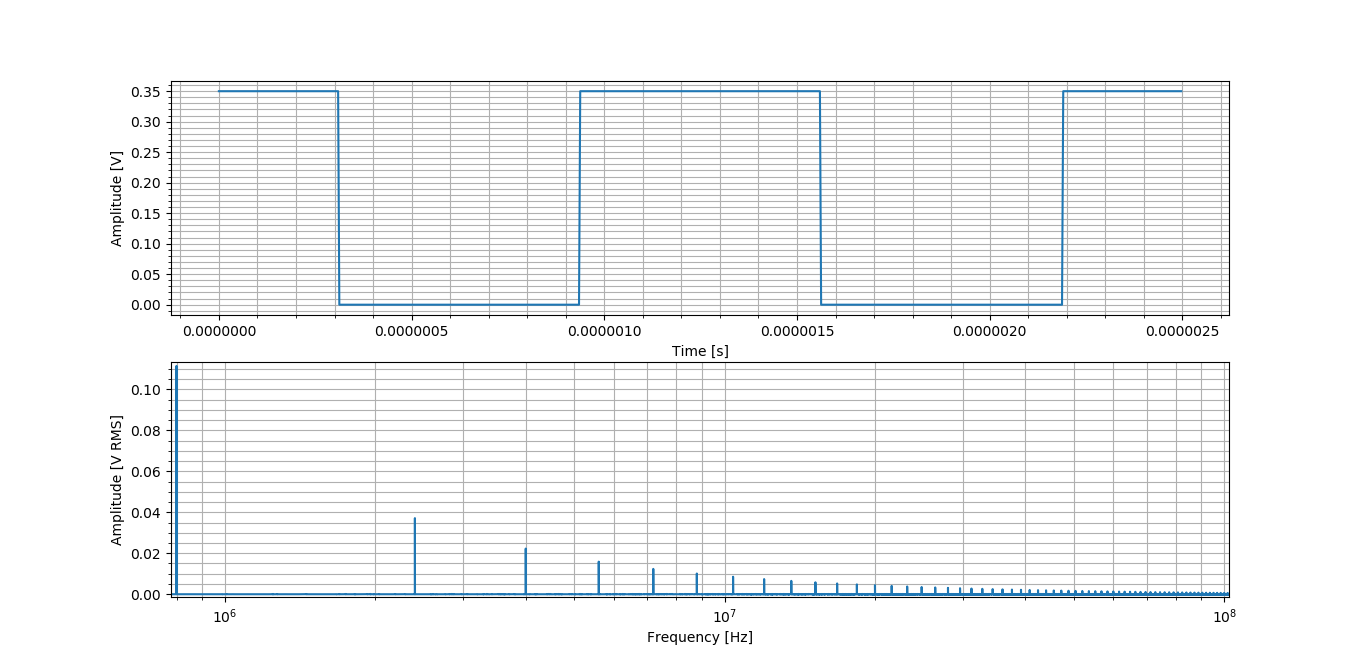
\includegraphics[scale=0.46]{Recursos/cuadrada_50_ejercicio_3.png}
    \caption{Diagrama espectral en magnitud de se\~nal cuadrada de  $50\%$ de duty}
\end{figure}

\begin{figure}[H]
    \centering
    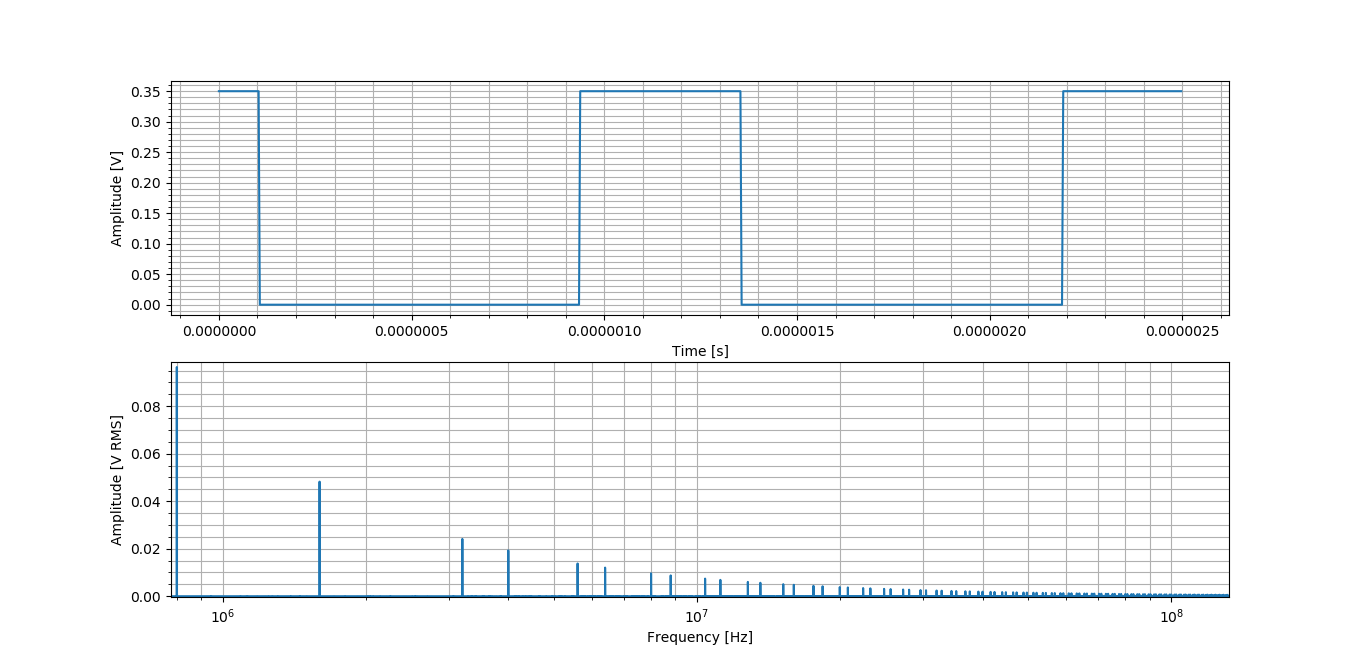
\includegraphics[scale=0.46]{Recursos/cuadrada_33_ejercicio_3.png}
    \caption{Diagrama espectral en magnitud de se\~nal cuadrada de  $33\%$ de duty}
\end{figure}

\begin{figure}[H]
    \centering
    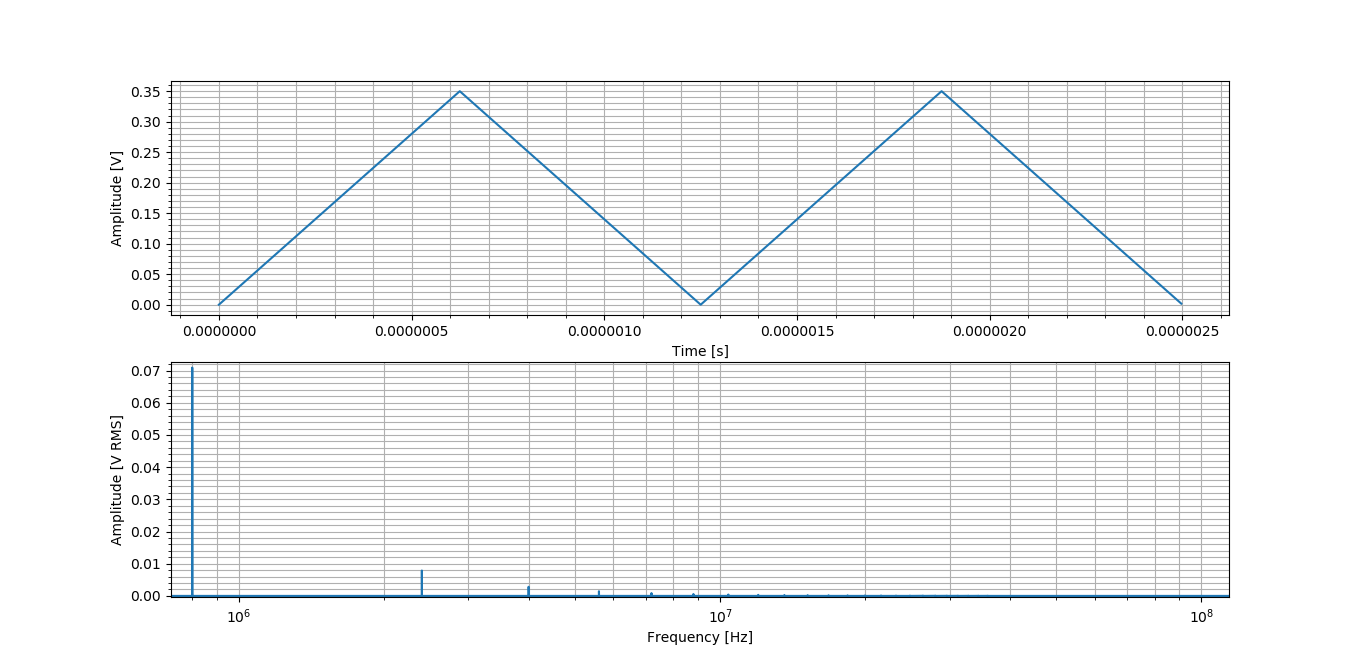
\includegraphics[scale=0.46]{Recursos/triangular_50_ejercicio_3.png}
    \caption{Diagrama espectral en magnitud de se\~nal triangular de  $50\%$ de duty}
\end{figure}

\subsection{Mediciones}

\begin{figure}[H]
    \centering
    \begin{tabular}{c c}
        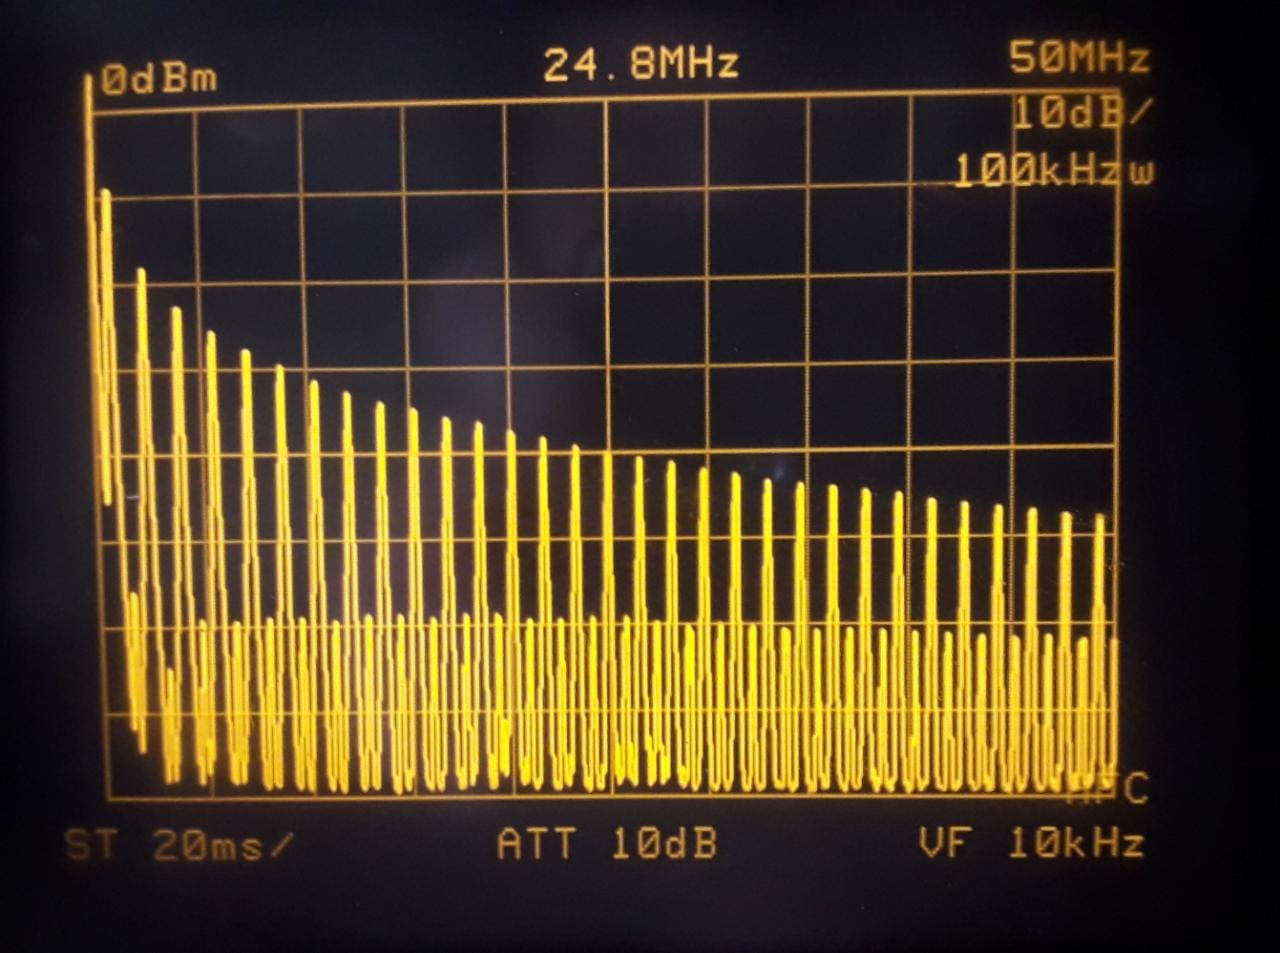
\includegraphics[scale=0.19]{../Mediciones/Ejercicio_2/ej2_cuadrada_50.jpeg} &
        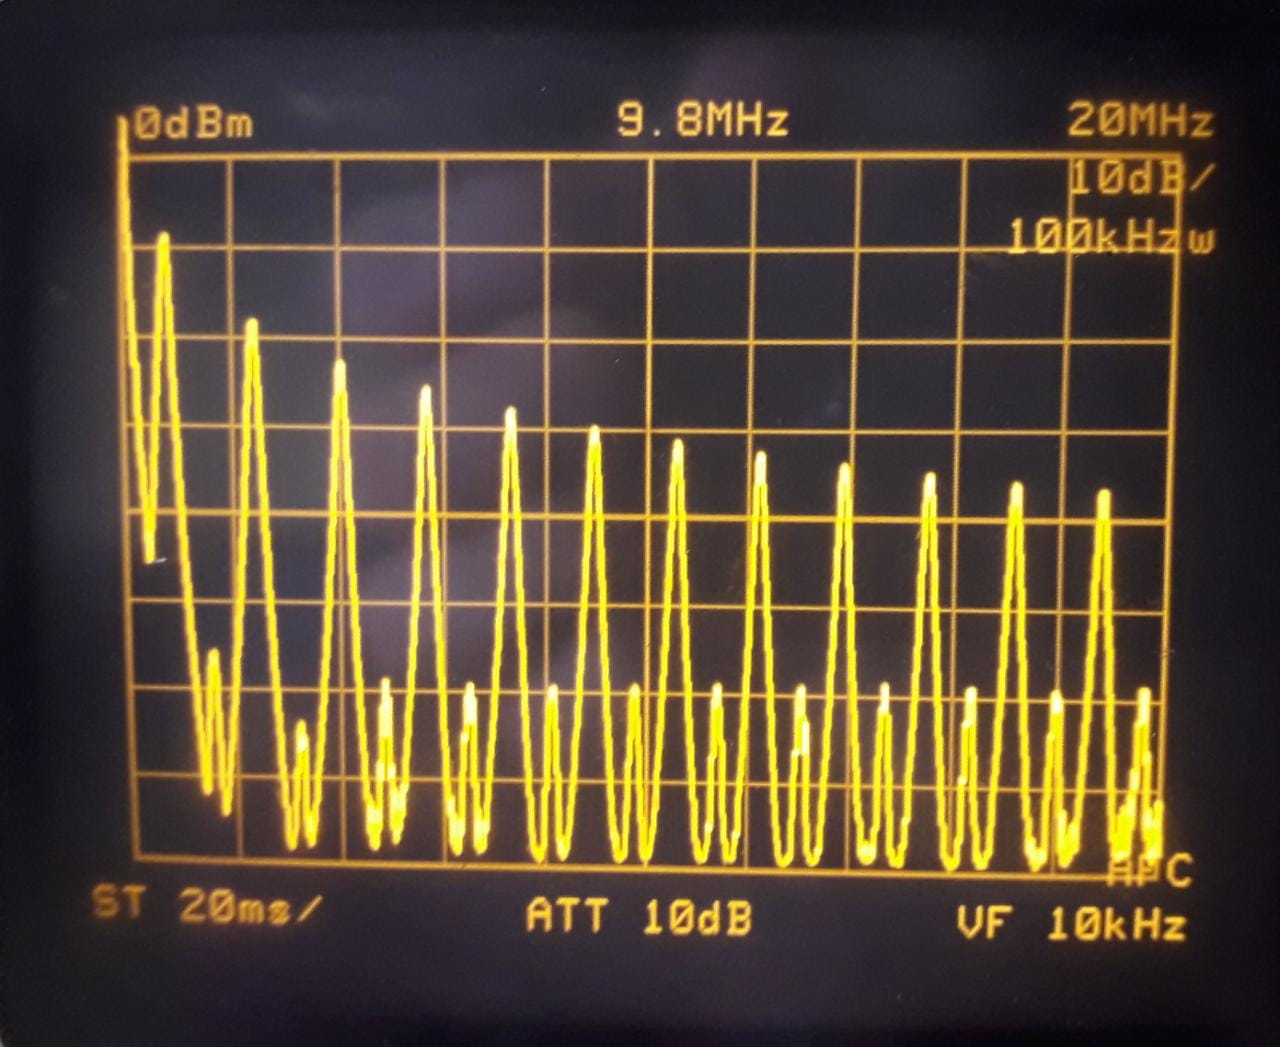
\includegraphics[scale=0.175]{../Mediciones/Ejercicio_2/ej2_cuadrada_50_zoom.jpeg}
    \end{tabular}
    \caption{Espectro de onda cuadrada de 800kHz, 350mVpp y 50$\%$}
    \label{ej2_cuadrada_50}
\end{figure}

\begin{figure}[H]
    \centering
    \begin{tabular}{c c}
        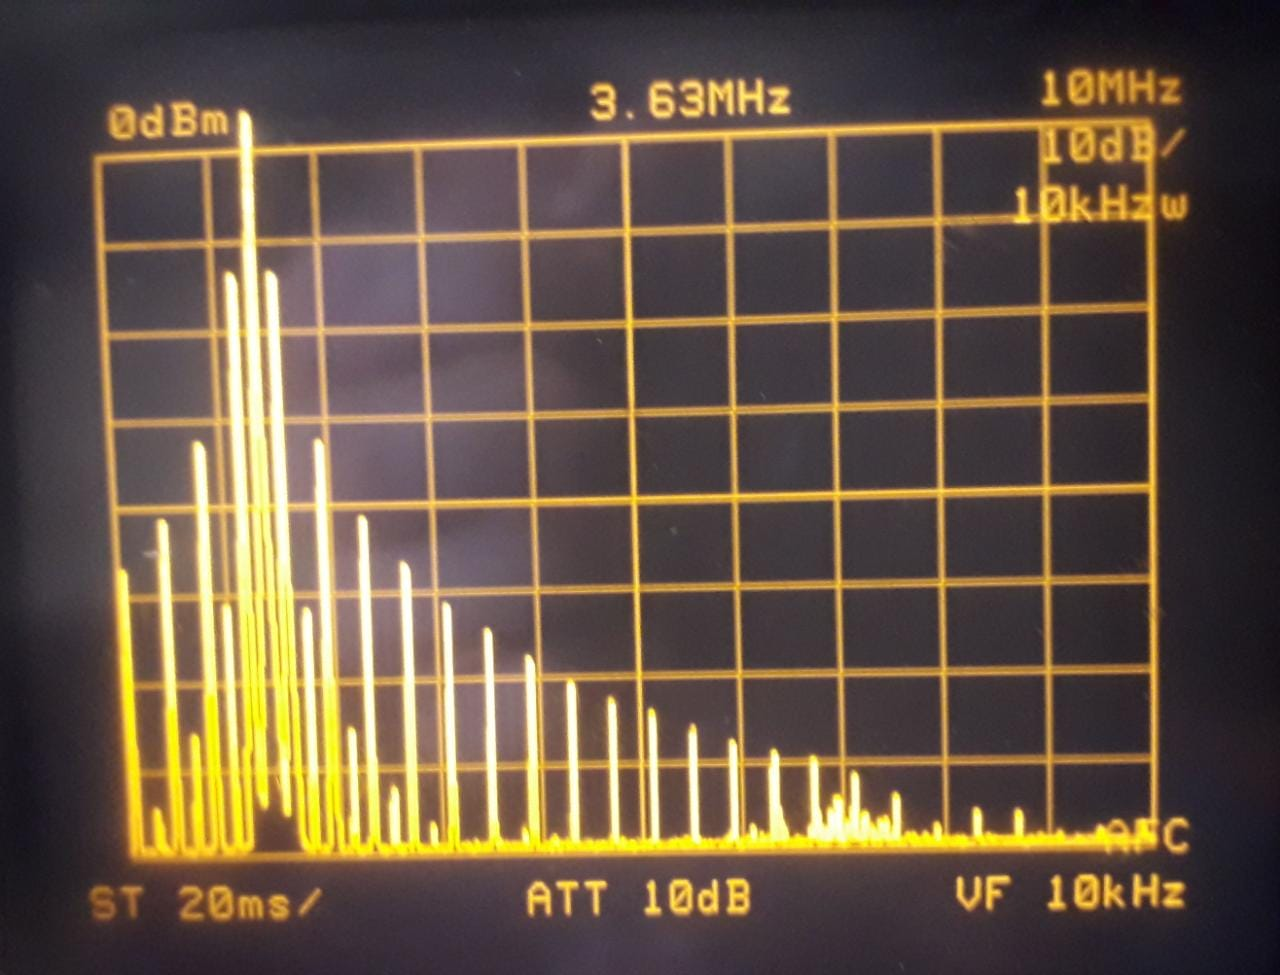
\includegraphics[scale=0.18]{../Mediciones/Ejercicio_2/ej2_triangular_50.jpeg} &
        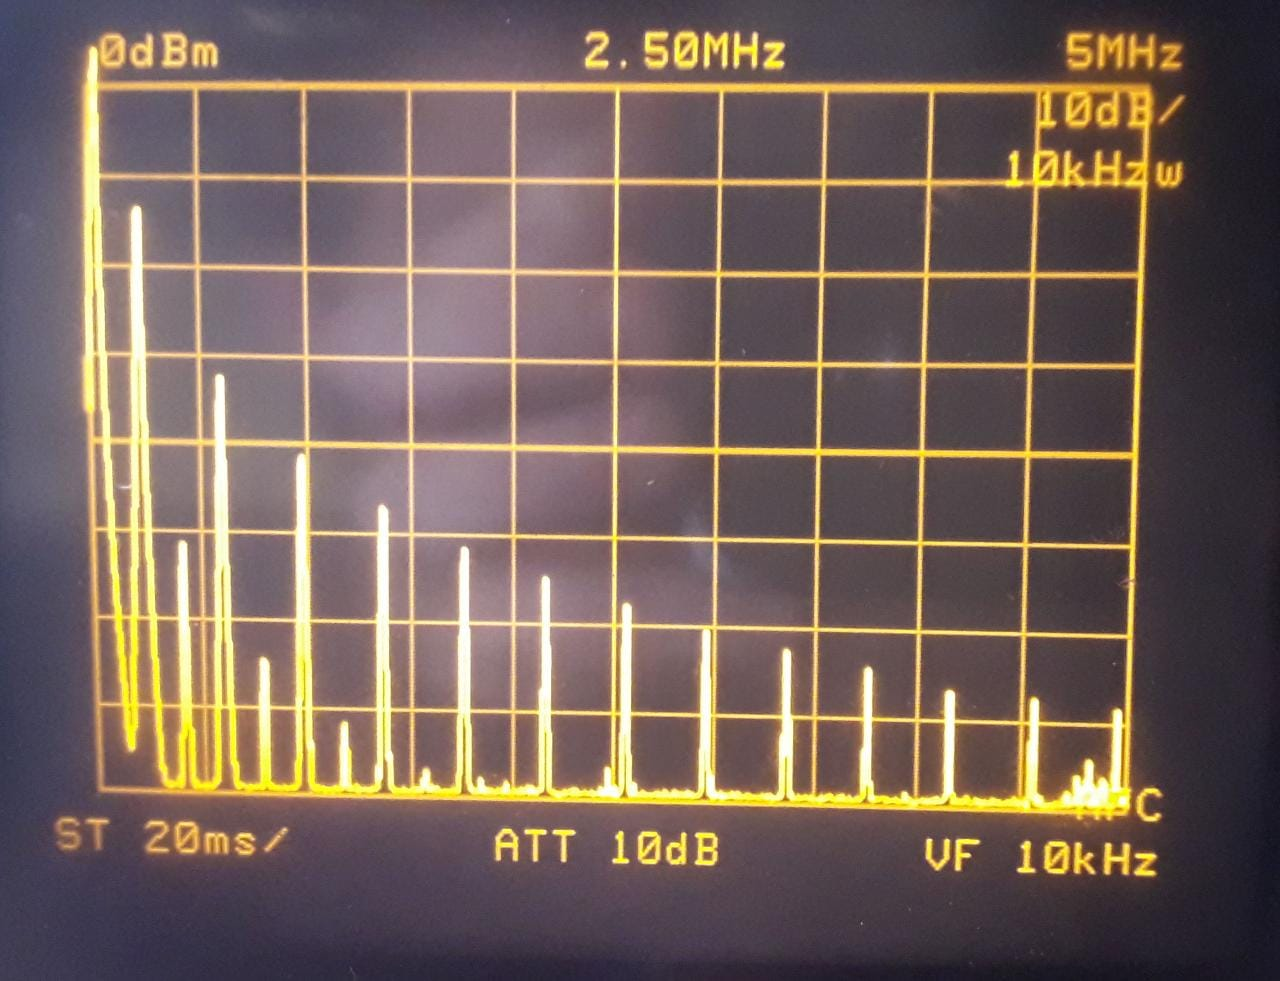
\includegraphics[scale=0.18]{../Mediciones/Ejercicio_2/ej2_triangular_50_zoom.jpeg}
    \end{tabular}
    \caption{Espectro de onda triangular de 800kHz, 350mVpp y 50$\%$}
    \label{ej2_triangular_50}
\end{figure}

\begin{figure}[H]
    \centering
    \begin{tabular}{c c}
        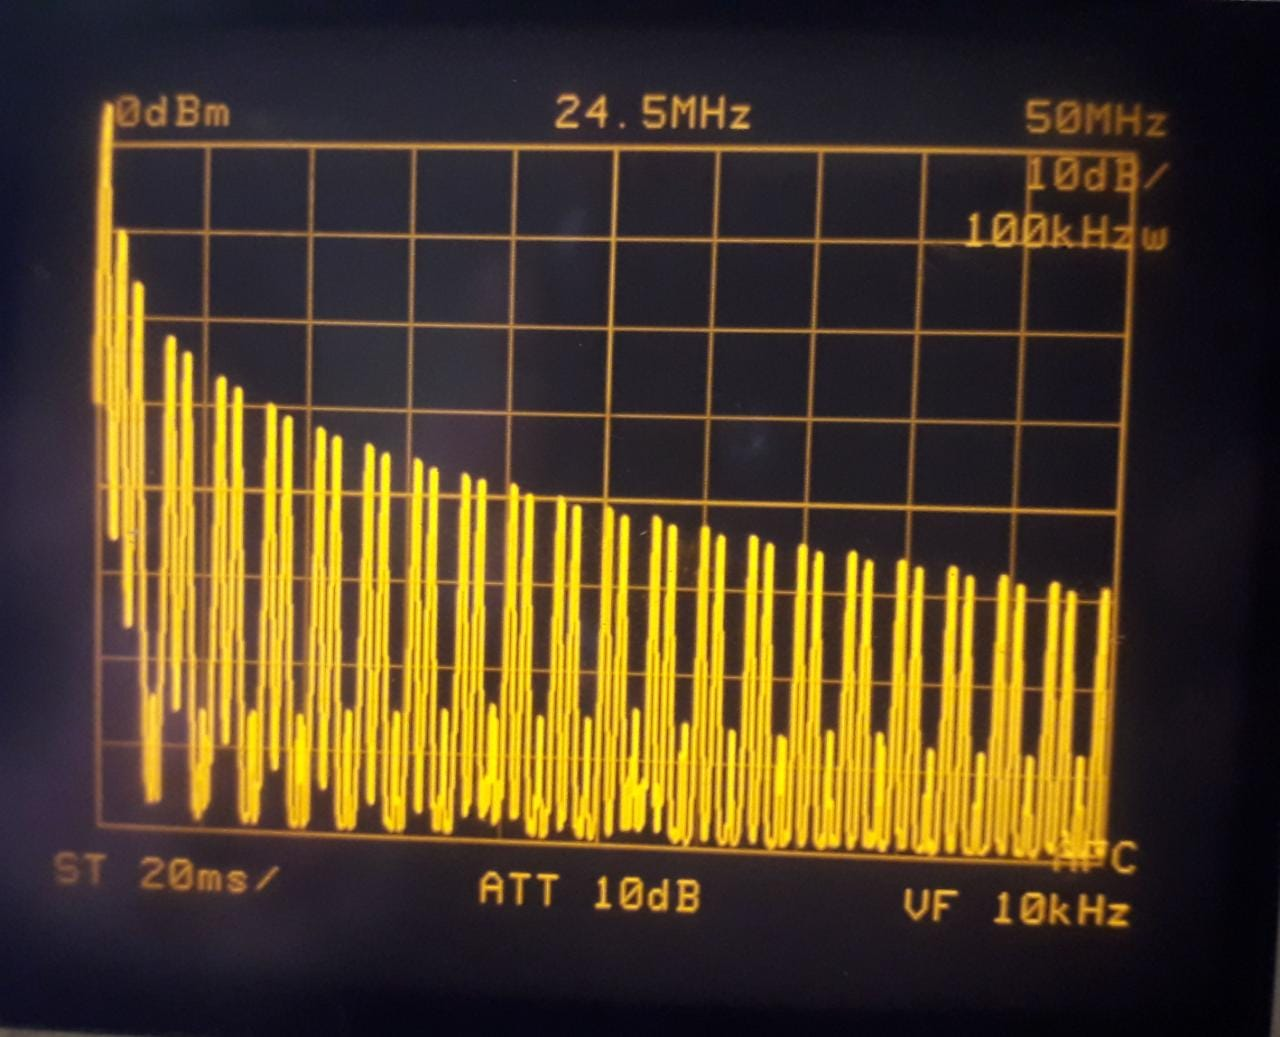
\includegraphics[scale=0.16]{../Mediciones/Ejercicio_2/ej2_cuadrada_33.jpeg} &
        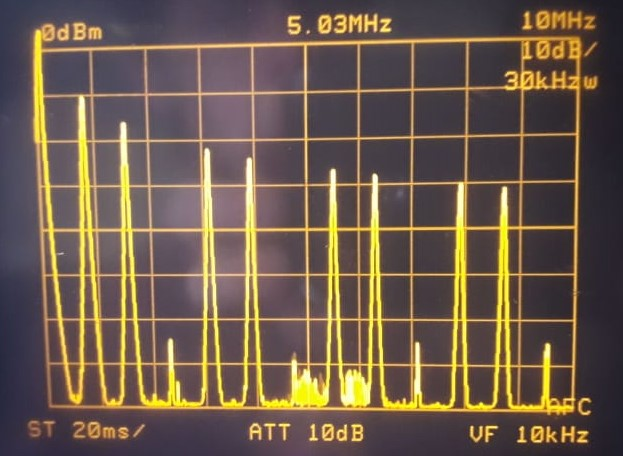
\includegraphics[scale=0.5]{../Mediciones/Ejercicio_2/ej2_cuadrada_33_zoom.jpeg}
    \end{tabular}
    \caption{Espectro de onda cuadrada de 800kHz, 350mVpp y 33$\%$}
    \label{ej2_cuadrada_33}
\end{figure}

\subsection{An\'alisis de los resultados}
A partir de las mediciones del espectro, y realizando una medici\'on de amplitudes relativas de los componentes arm\'onicos con respecto al fundamental,
utilizando la opci\'on Marker del analizador de espectro, se midieron sus valores de tensi\'on en dBm y realizando la conversi\'on y empleando la f\'ormula
obtenida en el an\'alisis te\'orico, se encontr\'o para cada caso el duty correspondiente.

En la Ec. \ref{eq:trasnformada_tren_pulsos} se puede observar una expresi\'on donde todos los componentes arm\'onicos est\'an en funci\'on del duty cycle de la onda
cuadrada y de all\'i se puede despejar para obtener los siguientes resultados. Esta operaci\'on consiste en evaluar:

\begin{align*}
    & a_n = A \cdot \frac{ \sin{\left( \pi \cdot n \cdot DC \right)} }{\pi \cdot n} \\
    & a_0 = A \cdot DC
\end{align*}
 
\begin{table}[H]
    \centering
    \begin{tabular}{c c c c}
        Amplitud [V] & Fundamental [dBm] & Duty Calculado \\
        \hline \\
        $188mV$ & $-10$ & $53.2 \%$ \\
        $188mV$ & $-14$ & $33.5 \%$\\
        \hline \\
    \end{tabular}
    \caption{Medici\'on del arm\'onico}
\end{table}
